\documentclass[twoside]{book}

% Packages required by doxygen
\usepackage{calc}
\usepackage{doxygen}
\usepackage{graphicx}
\usepackage[utf8]{inputenc}
\usepackage{makeidx}
\usepackage{multicol}
\usepackage{multirow}
\usepackage{textcomp}
\usepackage[table]{xcolor}

% Font selection
\usepackage[T1]{fontenc}
\usepackage{mathptmx}
\usepackage[scaled=.90]{helvet}
\usepackage{courier}
\usepackage{amssymb}
\usepackage{sectsty}
\renewcommand{\familydefault}{\sfdefault}
\allsectionsfont{%
  \fontseries{bc}\selectfont%
  \color{darkgray}%
}
\renewcommand{\DoxyLabelFont}{%
  \fontseries{bc}\selectfont%
  \color{darkgray}%
}

% Page & text layout
\usepackage{geometry}
\geometry{%
  a4paper,%
  top=2.5cm,%
  bottom=2.5cm,%
  left=2.5cm,%
  right=2.5cm%
}
\tolerance=750
\hfuzz=15pt
\hbadness=750
\setlength{\emergencystretch}{15pt}
\setlength{\parindent}{0cm}
\setlength{\parskip}{0.2cm}
\makeatletter
\renewcommand{\paragraph}{%
  \@startsection{paragraph}{4}{0ex}{-1.0ex}{1.0ex}{%
    \normalfont\normalsize\bfseries\SS@parafont%
  }%
}
\renewcommand{\subparagraph}{%
  \@startsection{subparagraph}{5}{0ex}{-1.0ex}{1.0ex}{%
    \normalfont\normalsize\bfseries\SS@subparafont%
  }%
}
\makeatother

% Headers & footers
\usepackage{fancyhdr}
\pagestyle{fancyplain}
\fancyhead[LE]{\fancyplain{}{\bfseries\thepage}}
\fancyhead[CE]{\fancyplain{}{}}
\fancyhead[RE]{\fancyplain{}{\bfseries\leftmark}}
\fancyhead[LO]{\fancyplain{}{\bfseries\rightmark}}
\fancyhead[CO]{\fancyplain{}{}}
\fancyhead[RO]{\fancyplain{}{\bfseries\thepage}}
\fancyfoot[LE]{\fancyplain{}{}}
\fancyfoot[CE]{\fancyplain{}{}}
\fancyfoot[RE]{\fancyplain{}{\bfseries\scriptsize Generated on Fri May 30 2014 03\-:56\-:37 for A\-\_\-star by Doxygen }}
\fancyfoot[LO]{\fancyplain{}{\bfseries\scriptsize Generated on Fri May 30 2014 03\-:56\-:37 for A\-\_\-star by Doxygen }}
\fancyfoot[CO]{\fancyplain{}{}}
\fancyfoot[RO]{\fancyplain{}{}}
\renewcommand{\footrulewidth}{0.4pt}
\renewcommand{\chaptermark}[1]{%
  \markboth{#1}{}%
}
\renewcommand{\sectionmark}[1]{%
  \markright{\thesection\ #1}%
}

% Indices & bibliography
\usepackage{natbib}
\usepackage[titles]{tocloft}
\setcounter{tocdepth}{3}
\setcounter{secnumdepth}{5}
\makeindex

% Hyperlinks (required, but should be loaded last)
\usepackage{ifpdf}
\ifpdf
  \usepackage[pdftex,pagebackref=true]{hyperref}
\else
  \usepackage[ps2pdf,pagebackref=true]{hyperref}
\fi
\hypersetup{%
  colorlinks=true,%
  linkcolor=blue,%
  citecolor=blue,%
  unicode%
}

% Custom commands
\newcommand{\clearemptydoublepage}{%
  \newpage{\pagestyle{empty}\cleardoublepage}%
}


%===== C O N T E N T S =====

\begin{document}

% Titlepage & ToC
\hypersetup{pageanchor=false}
\pagenumbering{roman}
\begin{titlepage}
\vspace*{7cm}
\begin{center}%
{\Large A\-\_\-star \\[1ex]\large 1.\-0 }\\
\vspace*{1cm}
{\large Generated by Doxygen 1.8.6}\\
\vspace*{0.5cm}
{\small Fri May 30 2014 03:56:37}\\
\end{center}
\end{titlepage}
\clearemptydoublepage
\tableofcontents
\clearemptydoublepage
\pagenumbering{arabic}
\hypersetup{pageanchor=true}

%--- Begin generated contents ---
\chapter{A\-\_\-star}
\label{index}\hypertarget{index}{}\begin{DoxyAuthor}{Author}
Pawel Zurek 
\end{DoxyAuthor}
\begin{DoxyDate}{Date}
16.\-03.\-2014 
\end{DoxyDate}
\begin{DoxyVersion}{Version}
1.\-1.\-b
\end{DoxyVersion}
Program umożliwia liczenie czasu trwania operacji wypelniania liczbami stosu / kolejki.\hypertarget{index_etykieta-wazne-cechy}{}\section{Najważniejsze cechy}\label{index_etykieta-wazne-cechy}
Program sluzy do liczenia czasu wypelnienia liczbami stosow i kolejek za pomoca \-:\par


\par
-\/$>$ list \par
-\/$>$ tablic ( po przekroczeniu rozmiaru tablicy, rozmiar powiekszany o jeden ) \par
-\/$>$ tablic ( po przekroczeniu rozmiaru tablicy, rozmiar zwiekszany dwukrotnie )\hypertarget{index_etykieta-op-algorytm}{}\section{Opis algorytmu}\label{index_etykieta-op-algorytm}
Algorytm w tym zadaniu to 6 petli \-: \par
-\/$>$ wypelnienie stosu za pomoca listy \par
-\/$>$ wypelnienie kolejki za pomoca listy \par
-\/$>$ wypelnienie stosu za pomoca tablicy ( rozmiar o jeden ) \par
-\/$>$ wypelnienie stosu za pomoca tablicy ( rozmiar x2 ) \par
-\/$>$ wypelnienie kolejki za pomoca tablicy ( rozmiar o jeden ) \par
-\/$>$ wypelnienie kolejki za pomoca tablicy ( rozmiar x2)

\par
,na ktora sklada sie wypelnienie nastepujaca iloscia elementow\-:

\par
-\/$>$ 10 \par
-\/$>$ 100 \par
-\/$>$ 1000 \par
-\/$>$ 10000

Czasy sa wyprowadzane na standartowe wyjscie. 
\chapter{Class Index}
\section{Class List}
Here are the classes, structs, unions and interfaces with brief descriptions\-:\begin{DoxyCompactList}
\item\contentsline{section}{\hyperlink{class_graf}{Graf} \\*Modeluje pojecie graf. Klasa sluzy glownie do wykonania algorytmu wyszukiwania, czyli znalezienia polaczenia miedzy dwoma punktami }{\pageref{class_graf}}{}
\item\contentsline{section}{\hyperlink{structpor}{por} \\*Struktura porownywania Struktura ta ma na celu ulatwienie dzialania algorytmu wyszukiwania ( Dijkstry ) Prownuje ona wartosci drogi miedzy dwoma wezlami }{\pageref{structpor}}{}
\item\contentsline{section}{\hyperlink{struct_wezel}{Wezel} \\*Struktura Wezla Struktura ta ma zdefiniowane dwie zmienne nr oraz g, ktore odpowiadaja za przechowywanie numer wierzcholkana oraz droge jaka juz przebyl od poczatku dzialania wyszukiwania }{\pageref{struct_wezel}}{}
\item\contentsline{section}{\hyperlink{class_wierzcholek}{Wierzcholek} \\*Definicje dla klasy \hyperlink{class_wierzcholek}{Wierzcholek} Struktura ta ma zdefiniowane dwie zmienne sasiad oraz waga. Przy wczytywaniu pliku dodajac wierzcholek dodajemy odrazu informacje o aktualnym sasiedzie oraz o wadze polaczenia miedzy wierzcholkiem i sasiadem }{\pageref{class_wierzcholek}}{}
\end{DoxyCompactList}

\chapter{File Index}
\section{File List}
Here is a list of all files with brief descriptions\-:\begin{DoxyCompactList}
\item\contentsline{section}{/home/pawel/\-Dokumenty/programowanie/pamsi/projekt\-\_\-znajomi/prj/inc/\hyperlink{_dijkstry_8hh}{Dijkstry.\-hh} \\*Definicje funkcji dla klasy graf }{\pageref{_dijkstry_8hh}}{}
\item\contentsline{section}{/home/pawel/\-Dokumenty/programowanie/pamsi/projekt\-\_\-znajomi/prj/src/\hyperlink{_dijkstry_8cpp}{Dijkstry.\-cpp} \\*Plik zawiera funkcje z klasy graf }{\pageref{_dijkstry_8cpp}}{}
\item\contentsline{section}{/home/pawel/\-Dokumenty/programowanie/pamsi/projekt\-\_\-znajomi/prj/src/\hyperlink{main_8cpp}{main.\-cpp} \\*Plik zawiera funkcje \hyperlink{main_8cpp_ae66f6b31b5ad750f1fe042a706a4e3d4}{main()} }{\pageref{main_8cpp}}{}
\end{DoxyCompactList}

\chapter{Class Documentation}
\hypertarget{classbenchmark}{\section{benchmark Class Reference}
\label{classbenchmark}\index{benchmark@{benchmark}}
}


Modeluje pojecie Benchmark.  




{\ttfamily \#include $<$benchmark.\-hh$>$}

\subsection*{Public Member Functions}
\begin{DoxyCompactItemize}
\item 
\hyperlink{classbenchmark_af56f1d9420c5c1ccc65e4f6aac54658d}{benchmark} ()
\begin{DoxyCompactList}\small\item\em Konstruktor klasy Benchmark. \end{DoxyCompactList}\item 
void \hyperlink{classbenchmark_a42ab532c49030406366e859f9b3f29f8}{czas\-\_\-start} ()
\begin{DoxyCompactList}\small\item\em Funkcja pomocnicza mierzenia czasu. \end{DoxyCompactList}\item 
void \hyperlink{classbenchmark_a9beb25d3e65b94c1ac7c085d8105fe65}{czas\-\_\-stop} ()
\begin{DoxyCompactList}\small\item\em Funkcja pomocnicza mierzenia czasu. \end{DoxyCompactList}\item 
double \hyperlink{classbenchmark_a613a8792feca7c2622355922d64d6fcd}{ile\-\_\-czasu} ()
\begin{DoxyCompactList}\small\item\em Funkcja obliczania czasu dzialania programu. \end{DoxyCompactList}\item 
void \hyperlink{classbenchmark_a845da6947383df74d871e273bf225721}{wykonaj\-\_\-algorytn\-\_\-sortowanie} ()
\begin{DoxyCompactList}\small\item\em Funkcja wykonujaca algorytm. \end{DoxyCompactList}\item 
void \hyperlink{classbenchmark_aedc5a477317912eb0d9ca5f9f1da3b7c}{algorytm} ()
\begin{DoxyCompactList}\small\item\em Funkcja wykonujaca algorytm. \end{DoxyCompactList}\item 
void \hyperlink{classbenchmark_a45a6a3fcaf8d09f172f2776451d67c9b}{wyswietl\-\_\-wszystko} (double $\ast$c, double $\ast$q, double $\ast$m, double $\ast$h, int n, int s)
\begin{DoxyCompactList}\small\item\em Funkcja wyswietalnia wynikow. \end{DoxyCompactList}\end{DoxyCompactItemize}
\subsection*{Private Attributes}
\begin{DoxyCompactItemize}
\item 
double \hyperlink{classbenchmark_a90e6eda0144befd3f3bc1a881904fb57}{elapsed\-Time}
\begin{DoxyCompactList}\small\item\em Pole typu double, bedzie uzywane do mierzenia czasu dzialania pojedynczego wypelniania. \end{DoxyCompactList}\item 
double \hyperlink{classbenchmark_a563b747421276232836b7711b6881ec8}{czas}
\begin{DoxyCompactList}\small\item\em Pole typu double, bedzie uzywane do mierzenia calkowitego czasu dzialania programu. \end{DoxyCompactList}\item 
double \hyperlink{classbenchmark_af677300c0b0a0086f306a0a08a6172b9}{czas\-\_\-caly}
\begin{DoxyCompactList}\small\item\em Pole typu double, bedzie uzywane do mierzenia calkowitego czasu dzialania programu. ! \end{DoxyCompactList}\item 
timeval \hyperlink{classbenchmark_a7789217b36df3b3ae427ceaaa2694d0b}{t1}
\begin{DoxyCompactList}\small\item\em Pole typu timeval, pomoc do liczenia czasu dzialania operacji krotkich ( tzn pojedynczego dzialania) \end{DoxyCompactList}\item 
timeval \hyperlink{classbenchmark_aea9f22e585c0c5826329e48a97a99803}{t2}
\end{DoxyCompactItemize}


\subsection{Detailed Description}
Modeluje pojecie Benchmark. 

Klasa sluzy do przeprowadzenia Benchmarku programu, tzn \-: -\/$>$ wczytania dowolnego zestawu danych o ilosci elementow \-: \par
-\/$>$ 10 \par
-\/$>$ 100 \par
-\/$>$ 1000 \par
-\/$>$ 10000 \par
-\/$>$ 100000 \par
-\/$>$ 1000000 \par
 Trzema roznymi metodami \-: \par
 -\/$>$ Quick Sort \par
 -\/$>$ Merge Sort \par
 -\/$>$ Heap Sort \par
 Można jeszcze wybrać ile razy ma zostać wykonany program. \par
-\/$>$ Na koniec zostana wyswietlone czasy kazdej akcji z osobna oraz czas calkowity 

Definition at line 41 of file benchmark.\-hh.



\subsection{Constructor \& Destructor Documentation}
\hypertarget{classbenchmark_af56f1d9420c5c1ccc65e4f6aac54658d}{\index{benchmark@{benchmark}!benchmark@{benchmark}}
\index{benchmark@{benchmark}!benchmark@{benchmark}}
\subsubsection[{benchmark}]{\setlength{\rightskip}{0pt plus 5cm}benchmark\-::benchmark (
\begin{DoxyParamCaption}
{}
\end{DoxyParamCaption}
)\hspace{0.3cm}{\ttfamily [inline]}}}\label{classbenchmark_af56f1d9420c5c1ccc65e4f6aac54658d}


Konstruktor klasy Benchmark. 

Konstruktor jest bezparametryczny, inicjalizuje wszystkie skladowe klasy wartosciami zerowymi. 

Definition at line 71 of file benchmark.\-hh.



\subsection{Member Function Documentation}
\hypertarget{classbenchmark_aedc5a477317912eb0d9ca5f9f1da3b7c}{\index{benchmark@{benchmark}!algorytm@{algorytm}}
\index{algorytm@{algorytm}!benchmark@{benchmark}}
\subsubsection[{algorytm}]{\setlength{\rightskip}{0pt plus 5cm}void benchmark\-::algorytm (
\begin{DoxyParamCaption}
{}
\end{DoxyParamCaption}
)}}\label{classbenchmark_aedc5a477317912eb0d9ca5f9f1da3b7c}


Funkcja wykonujaca algorytm. 

Wykonanie algorytmu ma przebieg \-:\par
 -\/$>$ posortowanie wybranego pliku trzema metodami\-: \par

\begin{DoxyItemize}
\item Quick Sort
\item Merge Sort
\item Heap Sort -\/$>$ po każdym posortowaniu, obiekt jest całkowicie zerowany\par
 -\/$>$ wszystko to wykonuje się zadana przez uzytkownika ilosc razy \par
 
\end{DoxyItemize}

Definition at line 98 of file benchmark.\-cpp.



Here is the call graph for this function\-:\nopagebreak
\begin{figure}[H]
\begin{center}
\leavevmode
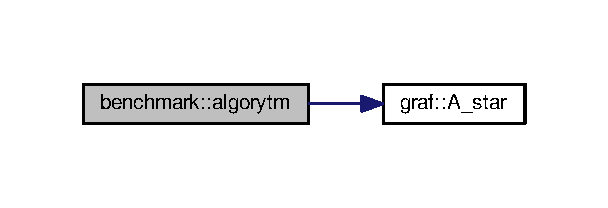
\includegraphics[width=350pt]{classbenchmark_aedc5a477317912eb0d9ca5f9f1da3b7c_cgraph}
\end{center}
\end{figure}




Here is the caller graph for this function\-:\nopagebreak
\begin{figure}[H]
\begin{center}
\leavevmode
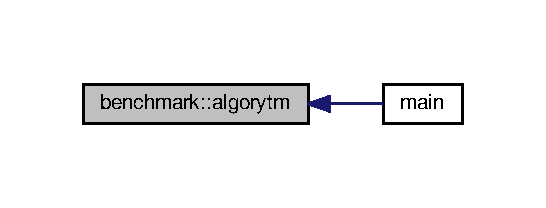
\includegraphics[width=262pt]{classbenchmark_aedc5a477317912eb0d9ca5f9f1da3b7c_icgraph}
\end{center}
\end{figure}


\hypertarget{classbenchmark_a42ab532c49030406366e859f9b3f29f8}{\index{benchmark@{benchmark}!czas\-\_\-start@{czas\-\_\-start}}
\index{czas\-\_\-start@{czas\-\_\-start}!benchmark@{benchmark}}
\subsubsection[{czas\-\_\-start}]{\setlength{\rightskip}{0pt plus 5cm}void benchmark\-::czas\-\_\-start (
\begin{DoxyParamCaption}
{}
\end{DoxyParamCaption}
)}}\label{classbenchmark_a42ab532c49030406366e859f9b3f29f8}


Funkcja pomocnicza mierzenia czasu. 

Funkcja zaczyna liczyc czas od momentu wywolania tej metody Sluzy do liczenia czasu wykonywania pojedynczego wypelniania stosu/kolejki 

Definition at line 14 of file benchmark.\-cpp.

\hypertarget{classbenchmark_a9beb25d3e65b94c1ac7c085d8105fe65}{\index{benchmark@{benchmark}!czas\-\_\-stop@{czas\-\_\-stop}}
\index{czas\-\_\-stop@{czas\-\_\-stop}!benchmark@{benchmark}}
\subsubsection[{czas\-\_\-stop}]{\setlength{\rightskip}{0pt plus 5cm}void benchmark\-::czas\-\_\-stop (
\begin{DoxyParamCaption}
{}
\end{DoxyParamCaption}
)}}\label{classbenchmark_a9beb25d3e65b94c1ac7c085d8105fe65}


Funkcja pomocnicza mierzenia czasu. 

Funkcja konczy liczyc czas od momentu wywolania tej metody Sluzy do liczenia czasu wykonywania pojedynczego wypelniania stosu/kolejki 

Definition at line 17 of file benchmark.\-cpp.

\hypertarget{classbenchmark_a613a8792feca7c2622355922d64d6fcd}{\index{benchmark@{benchmark}!ile\-\_\-czasu@{ile\-\_\-czasu}}
\index{ile\-\_\-czasu@{ile\-\_\-czasu}!benchmark@{benchmark}}
\subsubsection[{ile\-\_\-czasu}]{\setlength{\rightskip}{0pt plus 5cm}double benchmark\-::ile\-\_\-czasu (
\begin{DoxyParamCaption}
{}
\end{DoxyParamCaption}
)}}\label{classbenchmark_a613a8792feca7c2622355922d64d6fcd}


Funkcja obliczania czasu dzialania programu. 

Funkcja podaje czas wykonywania pojedynczego wypelniania stosu/kolejki

\begin{DoxyReturn}{Returns}
elapsed\-Time -\/$>$ zmienna typu double ( wynik obliczen ) 
\end{DoxyReturn}


Definition at line 20 of file benchmark.\-cpp.

\hypertarget{classbenchmark_a845da6947383df74d871e273bf225721}{\index{benchmark@{benchmark}!wykonaj\-\_\-algorytn\-\_\-sortowanie@{wykonaj\-\_\-algorytn\-\_\-sortowanie}}
\index{wykonaj\-\_\-algorytn\-\_\-sortowanie@{wykonaj\-\_\-algorytn\-\_\-sortowanie}!benchmark@{benchmark}}
\subsubsection[{wykonaj\-\_\-algorytn\-\_\-sortowanie}]{\setlength{\rightskip}{0pt plus 5cm}void benchmark\-::wykonaj\-\_\-algorytn\-\_\-sortowanie (
\begin{DoxyParamCaption}
{}
\end{DoxyParamCaption}
)}}\label{classbenchmark_a845da6947383df74d871e273bf225721}


Funkcja wykonujaca algorytm. 

Wykonanie algorytmu ma przebieg \-:\par
 -\/$>$ posortowanie danych metoda Quick Sort\par
 -\/$>$ posortowanie danych metoda Merge Sort\par
 -\/$>$ posortowanie danych metoda Heap Sort\par
 \par
 Dla \-:\par

\begin{DoxyItemize}
\item 10 elementow \par

\item 100 elementow \par

\item 1000 elementow \par

\item 10000 elementow \par

\item 100000 elementow \par

\item 1000000 elementow \par
 
\end{DoxyItemize}

Definition at line 27 of file benchmark.\-cpp.



Here is the call graph for this function\-:\nopagebreak
\begin{figure}[H]
\begin{center}
\leavevmode
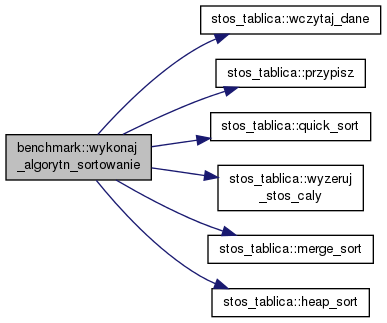
\includegraphics[width=350pt]{classbenchmark_a845da6947383df74d871e273bf225721_cgraph}
\end{center}
\end{figure}


\hypertarget{classbenchmark_a45a6a3fcaf8d09f172f2776451d67c9b}{\index{benchmark@{benchmark}!wyswietl\-\_\-wszystko@{wyswietl\-\_\-wszystko}}
\index{wyswietl\-\_\-wszystko@{wyswietl\-\_\-wszystko}!benchmark@{benchmark}}
\subsubsection[{wyswietl\-\_\-wszystko}]{\setlength{\rightskip}{0pt plus 5cm}void benchmark\-::wyswietl\-\_\-wszystko (
\begin{DoxyParamCaption}
\item[{double $\ast$}]{c, }
\item[{double $\ast$}]{q, }
\item[{double $\ast$}]{m, }
\item[{double $\ast$}]{h, }
\item[{int}]{n, }
\item[{int}]{s}
\end{DoxyParamCaption}
)}}\label{classbenchmark_a45a6a3fcaf8d09f172f2776451d67c9b}


Funkcja wyswietalnia wynikow. 

Funkcja wyswietla wszystkie czasy liczone w programie. Tzn\-: Czasy wszystkich wykonan dla kazdego sortowania, najwolniejsze, najszybsze oraz srednie wykonanie. Dodatkowo czas wykonania calej petli za kazdym razem


\begin{DoxyParams}{Parameters}
{\em c} & -\/$>$ wskaznik na zmienna typu double, przechowuje adres pola czasu calkowitego ( czasy ) \\
\hline
{\em q} & -\/$>$ wskaznik na zmienna typu double, przechowuje adres pola czasu wykonywania Quick Sort ( quick ) \\
\hline
{\em m} & -\/$>$ wskaznik na zmienna typu double, przechowuje adres pola czasu wykonywania Merge Sort ( merge ) \\
\hline
{\em h} & -\/$>$ wskaznik na zmienna typu double, przechowuje adres pola czasu wykonywania Heap Sort ( heap ) \\
\hline
{\em n} & -\/$>$ zmienna typu int, przechowuje adres pola, w ktorym jest informacja o tym ile razy zostal wykonany algorytm ( ile\-\_\-razy ) \\
\hline
{\em s} & -\/$>$ zmienna typu int, przechowuje adres pola rozmiaru tablicy ( size ) \\
\hline
\end{DoxyParams}


Definition at line 149 of file benchmark.\-cpp.



\subsection{Member Data Documentation}
\hypertarget{classbenchmark_a563b747421276232836b7711b6881ec8}{\index{benchmark@{benchmark}!czas@{czas}}
\index{czas@{czas}!benchmark@{benchmark}}
\subsubsection[{czas}]{\setlength{\rightskip}{0pt plus 5cm}double benchmark\-::czas\hspace{0.3cm}{\ttfamily [private]}}}\label{classbenchmark_a563b747421276232836b7711b6881ec8}


Pole typu double, bedzie uzywane do mierzenia calkowitego czasu dzialania programu. 



Definition at line 51 of file benchmark.\-hh.

\hypertarget{classbenchmark_af677300c0b0a0086f306a0a08a6172b9}{\index{benchmark@{benchmark}!czas\-\_\-caly@{czas\-\_\-caly}}
\index{czas\-\_\-caly@{czas\-\_\-caly}!benchmark@{benchmark}}
\subsubsection[{czas\-\_\-caly}]{\setlength{\rightskip}{0pt plus 5cm}double benchmark\-::czas\-\_\-caly\hspace{0.3cm}{\ttfamily [private]}}}\label{classbenchmark_af677300c0b0a0086f306a0a08a6172b9}


Pole typu double, bedzie uzywane do mierzenia calkowitego czasu dzialania programu. ! 



Definition at line 55 of file benchmark.\-hh.

\hypertarget{classbenchmark_a90e6eda0144befd3f3bc1a881904fb57}{\index{benchmark@{benchmark}!elapsed\-Time@{elapsed\-Time}}
\index{elapsed\-Time@{elapsed\-Time}!benchmark@{benchmark}}
\subsubsection[{elapsed\-Time}]{\setlength{\rightskip}{0pt plus 5cm}double benchmark\-::elapsed\-Time\hspace{0.3cm}{\ttfamily [private]}}}\label{classbenchmark_a90e6eda0144befd3f3bc1a881904fb57}


Pole typu double, bedzie uzywane do mierzenia czasu dzialania pojedynczego wypelniania. 



Definition at line 47 of file benchmark.\-hh.

\hypertarget{classbenchmark_a7789217b36df3b3ae427ceaaa2694d0b}{\index{benchmark@{benchmark}!t1@{t1}}
\index{t1@{t1}!benchmark@{benchmark}}
\subsubsection[{t1}]{\setlength{\rightskip}{0pt plus 5cm}timeval benchmark\-::t1\hspace{0.3cm}{\ttfamily [private]}}}\label{classbenchmark_a7789217b36df3b3ae427ceaaa2694d0b}


Pole typu timeval, pomoc do liczenia czasu dzialania operacji krotkich ( tzn pojedynczego dzialania) 



Definition at line 59 of file benchmark.\-hh.

\hypertarget{classbenchmark_aea9f22e585c0c5826329e48a97a99803}{\index{benchmark@{benchmark}!t2@{t2}}
\index{t2@{t2}!benchmark@{benchmark}}
\subsubsection[{t2}]{\setlength{\rightskip}{0pt plus 5cm}timeval benchmark\-::t2\hspace{0.3cm}{\ttfamily [private]}}}\label{classbenchmark_aea9f22e585c0c5826329e48a97a99803}


Definition at line 59 of file benchmark.\-hh.



The documentation for this class was generated from the following files\-:\begin{DoxyCompactItemize}
\item 
/home/pawel/\-Dokumenty/programowanie/pamsi/sortowaniev2/prj/inc/\hyperlink{benchmark_8hh}{benchmark.\-hh}\item 
/home/pawel/\-Dokumenty/programowanie/pamsi/sortowaniev2/prj/src/\hyperlink{benchmark_8cpp}{benchmark.\-cpp}\end{DoxyCompactItemize}

\hypertarget{classgraf}{\section{graf Class Reference}
\label{classgraf}\index{graf@{graf}}
}


Modeluje pojecie graf. Klasa sluzy glownie do wykonania algorytmu a\-\_\-star, czyli znalezienia najlepszej drogi miedzy dwoma punktami.  




{\ttfamily \#include $<$graf.\-hh$>$}



Collaboration diagram for graf\-:\nopagebreak
\begin{figure}[H]
\begin{center}
\leavevmode
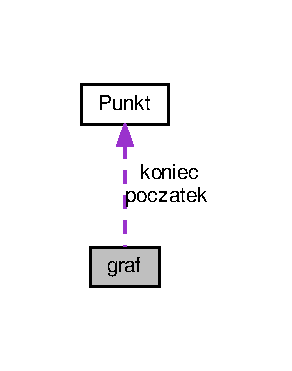
\includegraphics[width=140pt]{classgraf__coll__graph}
\end{center}
\end{figure}
\subsection*{Public Member Functions}
\begin{DoxyCompactItemize}
\item 
\hyperlink{classgraf_ae13560d84bcbc72d6aa0a10e94e245b6}{graf} (int rozmiar)
\begin{DoxyCompactList}\small\item\em Konstruktor klasy graf. \end{DoxyCompactList}\item 
void \hyperlink{classgraf_a0ccf7a033759840d0b63c9ab1eac79c3}{A\-\_\-star} ()
\begin{DoxyCompactList}\small\item\em Funkcja A\-\_\-star. Funkcja implementujaca algorytm przeszukiwania A\-\_\-star. Wywolywana bezparametrycznie, poniewaz punkt poczatkowy jak i koncowy ustalane sa w konstruktorze klasy graf. \end{DoxyCompactList}\end{DoxyCompactItemize}
\subsection*{Public Attributes}
\begin{DoxyCompactItemize}
\item 
vector$<$ vector$<$ \hyperlink{struct_wierzcholek}{Wierzcholek} $>$ $>$ \hyperlink{classgraf_a28ea2247c2bbe840ad2ad7f9fa98d596}{w}
\begin{DoxyCompactList}\small\item\em Pole typu vector$<$vector$<$$>$$>$, bedzie uzywane do przechowywania informacji o wierzcholku. \end{DoxyCompactList}\end{DoxyCompactItemize}
\subsection*{Private Member Functions}
\begin{DoxyCompactItemize}
\item 
void \hyperlink{classgraf_adb22c4f2d7a0f639cf121b87be24572c}{Stworz\-\_\-\-Sciane} (int start\-X, int start\-Y, int stop\-X, int stop\-Y)
\begin{DoxyCompactList}\small\item\em Funkcja tworzaca sciane. Funkcja tworzy sciane, przez ktora algorytm nie moze przejsc. Jest zmuszony do szukania drogi obok. \end{DoxyCompactList}\item 
void \hyperlink{classgraf_a932066fa342b0036a6580e797fa3a158}{Ustaw\-\_\-punkty} (int start\-X, int start\-Y, int stop\-X, int stop\-Y)
\begin{DoxyCompactList}\small\item\em Funkcja ustawiajace punkty do znalezienia. Funkcja ustala wspolrzedne punkty poczatkowego oraz koncowego. Nastepnie przydziela je do danego typu wierzcholka. \end{DoxyCompactList}\item 
void \hyperlink{classgraf_af93d38e243b89fd697acaf053752b154}{H} ()
\begin{DoxyCompactList}\small\item\em Funkcja heurestyczna. Funkcja oblicza przyblizona droge jaka algorytm musi przejsc, aby odnalezc cel. \end{DoxyCompactList}\item 
void \hyperlink{classgraf_ac8316d37401c007da5c583c80ee4de67}{G} ()
\begin{DoxyCompactList}\small\item\em Funkcja obliczajaca poniesiony. Funkcja oblicza koszt poniesiony miedzy wierzcholkiem poczatkowym a obecnym punktem. \end{DoxyCompactList}\item 
void \hyperlink{classgraf_adbcb36bc5251ca1c41a8b187edc39ded}{F} ()
\begin{DoxyCompactList}\small\item\em Funkcja obliczajaca wspolczynnik f. Wspolczynnik ten to suma arytmetyczna wspolczynnika g i h. Na podstawie tego algorytm A\-\_\-star wybiera wierzcholek o najnizszym wspolczynniku przez ktory przeszukuje graf. \end{DoxyCompactList}\item 
void \hyperlink{classgraf_ae5374a5a9711547b8afd136fad19f85b}{H} (\hyperlink{struct_punkt}{Punkt} \-\_\-w)
\begin{DoxyCompactList}\small\item\em Funkcja heurestyczna obliczajaca droge o zdanym punkcie. \end{DoxyCompactList}\item 
void \hyperlink{classgraf_ab9f67baa527bf9599a51c3496141ffec}{F} (\hyperlink{struct_punkt}{Punkt} \-\_\-w)
\begin{DoxyCompactList}\small\item\em Funkcja obliczajaca wspolczynnik f o zadanym punkcie. \end{DoxyCompactList}\item 
void \hyperlink{classgraf_a83ed10e2edea60ec7b8082d65dae0562}{Rozwiazanie} ()
\begin{DoxyCompactList}\small\item\em Funkcja interpretujaca rozwiazanie przeszukiwania przez algorytm. \end{DoxyCompactList}\end{DoxyCompactItemize}
\subsection*{Private Attributes}
\begin{DoxyCompactItemize}
\item 
\hyperlink{struct_punkt}{Punkt} \hyperlink{classgraf_a9472ec2485e3ab3363425b57b23972ae}{poczatek}
\begin{DoxyCompactList}\small\item\em Pole typu \hyperlink{struct_punkt}{Punkt}, bedzie uzywane do przechowywania informacji o punkcie poczatkowym. \end{DoxyCompactList}\item 
\hyperlink{struct_punkt}{Punkt} \hyperlink{classgraf_a484fe30b7f50d38d39bcb44d6ec88748}{koniec}
\begin{DoxyCompactList}\small\item\em Pole typu \hyperlink{struct_punkt}{Punkt}, bedzie uzywane do przechowywania informacji o punkcie koncowym. \end{DoxyCompactList}\end{DoxyCompactItemize}
\subsection*{Friends}
\begin{DoxyCompactItemize}
\item 
ostream \& \hyperlink{classgraf_a38651f35b4f57fd757770fcc914d3023}{operator$<$$<$} (ostream \&wyjscie, \hyperlink{classgraf}{graf} \&zmienna)
\begin{DoxyCompactList}\small\item\em Zdefiniowany operator wyswietlania Operator wypisuje na wyjsciu utworzone dane. \end{DoxyCompactList}\end{DoxyCompactItemize}


\subsection{Detailed Description}
Modeluje pojecie graf. Klasa sluzy glownie do wykonania algorytmu a\-\_\-star, czyli znalezienia najlepszej drogi miedzy dwoma punktami. 

Definition at line 93 of file graf.\-hh.



\subsection{Constructor \& Destructor Documentation}
\hypertarget{classgraf_ae13560d84bcbc72d6aa0a10e94e245b6}{\index{graf@{graf}!graf@{graf}}
\index{graf@{graf}!graf@{graf}}
\subsubsection[{graf}]{\setlength{\rightskip}{0pt plus 5cm}graf\-::graf (
\begin{DoxyParamCaption}
\item[{int}]{rozmiar}
\end{DoxyParamCaption}
)}}\label{classgraf_ae13560d84bcbc72d6aa0a10e94e245b6}


Konstruktor klasy graf. 

Konstruktor jest parametryczny. Parametrem tym jest rozmiar, ktory dediniuje rozmiar siatki i tym razem ilosc wierzcholkow ( rozmiar$^\wedge$2 ). Nastepnie pozwala ustawic sciane w dowolnym miejscu oraz dowolnie wybrac punkty \-: poczatkowy i koncowy. 
\begin{DoxyParams}{Parameters}
{\em rozmiar} & \\
\hline
\end{DoxyParams}


Definition at line 12 of file graf.\-cpp.



\subsection{Member Function Documentation}
\hypertarget{classgraf_a0ccf7a033759840d0b63c9ab1eac79c3}{\index{graf@{graf}!A\-\_\-star@{A\-\_\-star}}
\index{A\-\_\-star@{A\-\_\-star}!graf@{graf}}
\subsubsection[{A\-\_\-star}]{\setlength{\rightskip}{0pt plus 5cm}void graf\-::\-A\-\_\-star (
\begin{DoxyParamCaption}
{}
\end{DoxyParamCaption}
)}}\label{classgraf_a0ccf7a033759840d0b63c9ab1eac79c3}


Funkcja A\-\_\-star. Funkcja implementujaca algorytm przeszukiwania A\-\_\-star. Wywolywana bezparametrycznie, poniewaz punkt poczatkowy jak i koncowy ustalane sa w konstruktorze klasy graf. 



Definition at line 125 of file graf.\-cpp.



Here is the caller graph for this function\-:
\nopagebreak
\begin{figure}[H]
\begin{center}
\leavevmode
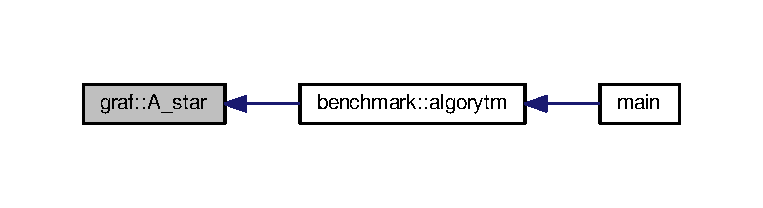
\includegraphics[width=350pt]{classgraf_a0ccf7a033759840d0b63c9ab1eac79c3_icgraph}
\end{center}
\end{figure}


\hypertarget{classgraf_adbcb36bc5251ca1c41a8b187edc39ded}{\index{graf@{graf}!F@{F}}
\index{F@{F}!graf@{graf}}
\subsubsection[{F}]{\setlength{\rightskip}{0pt plus 5cm}void graf\-::\-F (
\begin{DoxyParamCaption}
{}
\end{DoxyParamCaption}
)\hspace{0.3cm}{\ttfamily [private]}}}\label{classgraf_adbcb36bc5251ca1c41a8b187edc39ded}


Funkcja obliczajaca wspolczynnik f. Wspolczynnik ten to suma arytmetyczna wspolczynnika g i h. Na podstawie tego algorytm A\-\_\-star wybiera wierzcholek o najnizszym wspolczynniku przez ktory przeszukuje graf. 



Definition at line 98 of file graf.\-cpp.

\hypertarget{classgraf_ab9f67baa527bf9599a51c3496141ffec}{\index{graf@{graf}!F@{F}}
\index{F@{F}!graf@{graf}}
\subsubsection[{F}]{\setlength{\rightskip}{0pt plus 5cm}void graf\-::\-F (
\begin{DoxyParamCaption}
\item[{{\bf Punkt}}]{\-\_\-w}
\end{DoxyParamCaption}
)\hspace{0.3cm}{\ttfamily [private]}}}\label{classgraf_ab9f67baa527bf9599a51c3496141ffec}


Funkcja obliczajaca wspolczynnik f o zadanym punkcie. 


\begin{DoxyParams}{Parameters}
{\em \-\_\-w} & \\
\hline
\end{DoxyParams}


Definition at line 112 of file graf.\-cpp.

\hypertarget{classgraf_ac8316d37401c007da5c583c80ee4de67}{\index{graf@{graf}!G@{G}}
\index{G@{G}!graf@{graf}}
\subsubsection[{G}]{\setlength{\rightskip}{0pt plus 5cm}void graf\-::\-G (
\begin{DoxyParamCaption}
{}
\end{DoxyParamCaption}
)\hspace{0.3cm}{\ttfamily [private]}}}\label{classgraf_ac8316d37401c007da5c583c80ee4de67}


Funkcja obliczajaca poniesiony. Funkcja oblicza koszt poniesiony miedzy wierzcholkiem poczatkowym a obecnym punktem. 



Definition at line 88 of file graf.\-cpp.

\hypertarget{classgraf_af93d38e243b89fd697acaf053752b154}{\index{graf@{graf}!H@{H}}
\index{H@{H}!graf@{graf}}
\subsubsection[{H}]{\setlength{\rightskip}{0pt plus 5cm}void graf\-::\-H (
\begin{DoxyParamCaption}
{}
\end{DoxyParamCaption}
)\hspace{0.3cm}{\ttfamily [private]}}}\label{classgraf_af93d38e243b89fd697acaf053752b154}


Funkcja heurestyczna. Funkcja oblicza przyblizona droge jaka algorytm musi przejsc, aby odnalezc cel. 



Definition at line 78 of file graf.\-cpp.

\hypertarget{classgraf_ae5374a5a9711547b8afd136fad19f85b}{\index{graf@{graf}!H@{H}}
\index{H@{H}!graf@{graf}}
\subsubsection[{H}]{\setlength{\rightskip}{0pt plus 5cm}void graf\-::\-H (
\begin{DoxyParamCaption}
\item[{{\bf Punkt}}]{\-\_\-w}
\end{DoxyParamCaption}
)\hspace{0.3cm}{\ttfamily [private]}}}\label{classgraf_ae5374a5a9711547b8afd136fad19f85b}


Funkcja heurestyczna obliczajaca droge o zdanym punkcie. 


\begin{DoxyParams}{Parameters}
{\em \-\_\-w} & \\
\hline
\end{DoxyParams}


Definition at line 108 of file graf.\-cpp.

\hypertarget{classgraf_a83ed10e2edea60ec7b8082d65dae0562}{\index{graf@{graf}!Rozwiazanie@{Rozwiazanie}}
\index{Rozwiazanie@{Rozwiazanie}!graf@{graf}}
\subsubsection[{Rozwiazanie}]{\setlength{\rightskip}{0pt plus 5cm}void graf\-::\-Rozwiazanie (
\begin{DoxyParamCaption}
{}
\end{DoxyParamCaption}
)\hspace{0.3cm}{\ttfamily [private]}}}\label{classgraf_a83ed10e2edea60ec7b8082d65dae0562}


Funkcja interpretujaca rozwiazanie przeszukiwania przez algorytm. 



Definition at line 116 of file graf.\-cpp.

\hypertarget{classgraf_adb22c4f2d7a0f639cf121b87be24572c}{\index{graf@{graf}!Stworz\-\_\-\-Sciane@{Stworz\-\_\-\-Sciane}}
\index{Stworz\-\_\-\-Sciane@{Stworz\-\_\-\-Sciane}!graf@{graf}}
\subsubsection[{Stworz\-\_\-\-Sciane}]{\setlength{\rightskip}{0pt plus 5cm}void graf\-::\-Stworz\-\_\-\-Sciane (
\begin{DoxyParamCaption}
\item[{int}]{start\-X, }
\item[{int}]{start\-Y, }
\item[{int}]{stop\-X, }
\item[{int}]{stop\-Y}
\end{DoxyParamCaption}
)\hspace{0.3cm}{\ttfamily [private]}}}\label{classgraf_adb22c4f2d7a0f639cf121b87be24572c}


Funkcja tworzaca sciane. Funkcja tworzy sciane, przez ktora algorytm nie moze przejsc. Jest zmuszony do szukania drogi obok. 


\begin{DoxyParams}{Parameters}
{\em start\-X} & \\
\hline
{\em start\-Y} & \\
\hline
{\em stop\-X} & \\
\hline
{\em stop\-Y} & \\
\hline
\end{DoxyParams}


Definition at line 60 of file graf.\-cpp.

\hypertarget{classgraf_a932066fa342b0036a6580e797fa3a158}{\index{graf@{graf}!Ustaw\-\_\-punkty@{Ustaw\-\_\-punkty}}
\index{Ustaw\-\_\-punkty@{Ustaw\-\_\-punkty}!graf@{graf}}
\subsubsection[{Ustaw\-\_\-punkty}]{\setlength{\rightskip}{0pt plus 5cm}void graf\-::\-Ustaw\-\_\-punkty (
\begin{DoxyParamCaption}
\item[{int}]{start\-X, }
\item[{int}]{start\-Y, }
\item[{int}]{stop\-X, }
\item[{int}]{stop\-Y}
\end{DoxyParamCaption}
)\hspace{0.3cm}{\ttfamily [private]}}}\label{classgraf_a932066fa342b0036a6580e797fa3a158}


Funkcja ustawiajace punkty do znalezienia. Funkcja ustala wspolrzedne punkty poczatkowego oraz koncowego. Nastepnie przydziela je do danego typu wierzcholka. 


\begin{DoxyParams}{Parameters}
{\em start\-X} & \\
\hline
{\em start\-Y} & \\
\hline
{\em stop\-X} & \\
\hline
{\em stop\-Y} & \\
\hline
\end{DoxyParams}


Definition at line 71 of file graf.\-cpp.



\subsection{Friends And Related Function Documentation}
\hypertarget{classgraf_a38651f35b4f57fd757770fcc914d3023}{\index{graf@{graf}!operator$<$$<$@{operator$<$$<$}}
\index{operator$<$$<$@{operator$<$$<$}!graf@{graf}}
\subsubsection[{operator$<$$<$}]{\setlength{\rightskip}{0pt plus 5cm}ostream\& operator$<$$<$ (
\begin{DoxyParamCaption}
\item[{ostream \&}]{wyjscie, }
\item[{{\bf graf} \&}]{zmienna}
\end{DoxyParamCaption}
)\hspace{0.3cm}{\ttfamily [friend]}}}\label{classgraf_a38651f35b4f57fd757770fcc914d3023}


Zdefiniowany operator wyswietlania Operator wypisuje na wyjsciu utworzone dane. 

\begin{DoxyReturn}{Returns}
wyjscie 
\end{DoxyReturn}


Definition at line 175 of file graf.\-hh.



\subsection{Member Data Documentation}
\hypertarget{classgraf_a484fe30b7f50d38d39bcb44d6ec88748}{\index{graf@{graf}!koniec@{koniec}}
\index{koniec@{koniec}!graf@{graf}}
\subsubsection[{koniec}]{\setlength{\rightskip}{0pt plus 5cm}{\bf Punkt} graf\-::koniec\hspace{0.3cm}{\ttfamily [private]}}}\label{classgraf_a484fe30b7f50d38d39bcb44d6ec88748}


Pole typu \hyperlink{struct_punkt}{Punkt}, bedzie uzywane do przechowywania informacji o punkcie koncowym. 



Definition at line 101 of file graf.\-hh.

\hypertarget{classgraf_a9472ec2485e3ab3363425b57b23972ae}{\index{graf@{graf}!poczatek@{poczatek}}
\index{poczatek@{poczatek}!graf@{graf}}
\subsubsection[{poczatek}]{\setlength{\rightskip}{0pt plus 5cm}{\bf Punkt} graf\-::poczatek\hspace{0.3cm}{\ttfamily [private]}}}\label{classgraf_a9472ec2485e3ab3363425b57b23972ae}


Pole typu \hyperlink{struct_punkt}{Punkt}, bedzie uzywane do przechowywania informacji o punkcie poczatkowym. 



Definition at line 97 of file graf.\-hh.

\hypertarget{classgraf_a28ea2247c2bbe840ad2ad7f9fa98d596}{\index{graf@{graf}!w@{w}}
\index{w@{w}!graf@{graf}}
\subsubsection[{w}]{\setlength{\rightskip}{0pt plus 5cm}vector$<$ vector$<${\bf Wierzcholek}$>$ $>$ graf\-::w}}\label{classgraf_a28ea2247c2bbe840ad2ad7f9fa98d596}


Pole typu vector$<$vector$<$$>$$>$, bedzie uzywane do przechowywania informacji o wierzcholku. 



Definition at line 158 of file graf.\-hh.



The documentation for this class was generated from the following files\-:\begin{DoxyCompactItemize}
\item 
/home/pawel/\-Dokumenty/programowanie/pamsi/a\-\_\-star/prj/inc/\hyperlink{graf_8hh}{graf.\-hh}\item 
/home/pawel/\-Dokumenty/programowanie/pamsi/a\-\_\-star/prj/src/\hyperlink{graf_8cpp}{graf.\-cpp}\end{DoxyCompactItemize}

\hypertarget{struct_punkt}{\section{Punkt Struct Reference}
\label{struct_punkt}\index{Punkt@{Punkt}}
}


Struktura punktu Struktura ta ma zdefiniowane dwie zmienne x oraz y, ktore odpowiadaja za przechowywanie pozycji na siatce. Rowniez zdefiniowane sa operator przypisania oraz operator logiczny relacji.  




{\ttfamily \#include $<$graf.\-hh$>$}

\subsection*{Public Member Functions}
\begin{DoxyCompactItemize}
\item 
bool \hyperlink{struct_punkt_a93a161118cc9676368dbc7c4c9df86a0}{operator==} (\hyperlink{struct_punkt}{Punkt} wsp)
\begin{DoxyCompactList}\small\item\em Zdefiniowany operator porownania. Jezeli zmienne x i y sa rowne wspolrzednym tych zmiennych to zwracana jest wartosc 1. \end{DoxyCompactList}\item 
bool \hyperlink{struct_punkt_a47ca4abd0c2dbcd21a854b5056e5be6e}{operator!=} (\hyperlink{struct_punkt}{Punkt} wsp)
\begin{DoxyCompactList}\small\item\em Zdefiniowany operator relacji. \end{DoxyCompactList}\end{DoxyCompactItemize}
\subsection*{Public Attributes}
\begin{DoxyCompactItemize}
\item 
int \hyperlink{struct_punkt_a3c8936f679ef8fc4c1380ebc45820dc4}{x}
\begin{DoxyCompactList}\small\item\em Pole typu int, bedzie uzywane do przechowywania wspolrzednej x-\/owej. \end{DoxyCompactList}\item 
int \hyperlink{struct_punkt_a68c1591209ee35bec2189fb87cbe57bb}{y}
\begin{DoxyCompactList}\small\item\em Pole typu int, bedzie uzywane do przechowywania wspolrzednej y-\/kowej. \end{DoxyCompactList}\end{DoxyCompactItemize}


\subsection{Detailed Description}
Struktura punktu Struktura ta ma zdefiniowane dwie zmienne x oraz y, ktore odpowiadaja za przechowywanie pozycji na siatce. Rowniez zdefiniowane sa operator przypisania oraz operator logiczny relacji. 

Definition at line 38 of file graf.\-hh.



\subsection{Member Function Documentation}
\hypertarget{struct_punkt_a47ca4abd0c2dbcd21a854b5056e5be6e}{\index{Punkt@{Punkt}!operator!=@{operator!=}}
\index{operator!=@{operator!=}!Punkt@{Punkt}}
\subsubsection[{operator!=}]{\setlength{\rightskip}{0pt plus 5cm}bool Punkt\-::operator!= (
\begin{DoxyParamCaption}
\item[{{\bf Punkt}}]{wsp}
\end{DoxyParamCaption}
)\hspace{0.3cm}{\ttfamily [inline]}}}\label{struct_punkt_a47ca4abd0c2dbcd21a854b5056e5be6e}


Zdefiniowany operator relacji. 



Definition at line 59 of file graf.\-hh.

\hypertarget{struct_punkt_a93a161118cc9676368dbc7c4c9df86a0}{\index{Punkt@{Punkt}!operator==@{operator==}}
\index{operator==@{operator==}!Punkt@{Punkt}}
\subsubsection[{operator==}]{\setlength{\rightskip}{0pt plus 5cm}bool Punkt\-::operator== (
\begin{DoxyParamCaption}
\item[{{\bf Punkt}}]{wsp}
\end{DoxyParamCaption}
)\hspace{0.3cm}{\ttfamily [inline]}}}\label{struct_punkt_a93a161118cc9676368dbc7c4c9df86a0}


Zdefiniowany operator porownania. Jezeli zmienne x i y sa rowne wspolrzednym tych zmiennych to zwracana jest wartosc 1. 



Definition at line 52 of file graf.\-hh.



\subsection{Member Data Documentation}
\hypertarget{struct_punkt_a3c8936f679ef8fc4c1380ebc45820dc4}{\index{Punkt@{Punkt}!x@{x}}
\index{x@{x}!Punkt@{Punkt}}
\subsubsection[{x}]{\setlength{\rightskip}{0pt plus 5cm}int Punkt\-::x}}\label{struct_punkt_a3c8936f679ef8fc4c1380ebc45820dc4}


Pole typu int, bedzie uzywane do przechowywania wspolrzednej x-\/owej. 



Definition at line 43 of file graf.\-hh.

\hypertarget{struct_punkt_a68c1591209ee35bec2189fb87cbe57bb}{\index{Punkt@{Punkt}!y@{y}}
\index{y@{y}!Punkt@{Punkt}}
\subsubsection[{y}]{\setlength{\rightskip}{0pt plus 5cm}int Punkt\-::y}}\label{struct_punkt_a68c1591209ee35bec2189fb87cbe57bb}


Pole typu int, bedzie uzywane do przechowywania wspolrzednej y-\/kowej. 



Definition at line 47 of file graf.\-hh.



The documentation for this struct was generated from the following file\-:\begin{DoxyCompactItemize}
\item 
/home/pawel/\-Dokumenty/programowanie/pamsi/a\-\_\-star/prj/inc/\hyperlink{graf_8hh}{graf.\-hh}\end{DoxyCompactItemize}

\hypertarget{struct_wierzcholek}{\section{Wierzcholek Struct Reference}
\label{struct_wierzcholek}\index{Wierzcholek@{Wierzcholek}}
}


Struktura \hyperlink{struct_wierzcholek}{Wierzcholek}. Opisuje wlasnosci wierzcholka.  




{\ttfamily \#include $<$graf.\-hh$>$}



Collaboration diagram for Wierzcholek\-:\nopagebreak
\begin{figure}[H]
\begin{center}
\leavevmode
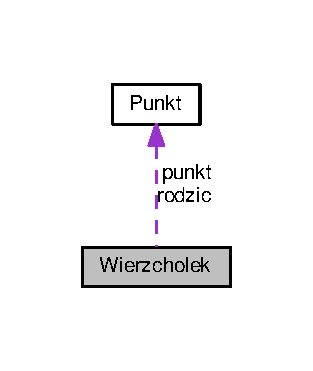
\includegraphics[width=150pt]{struct_wierzcholek__coll__graph}
\end{center}
\end{figure}
\subsection*{Public Attributes}
\begin{DoxyCompactItemize}
\item 
\hyperlink{graf_8hh_af54d448689b4613c3715929ca2a914a2}{Wierzcholek\-\_\-\-Typ} \hyperlink{struct_wierzcholek_ac812fe482bda5f924cf38d48340aa018}{typ}
\begin{DoxyCompactList}\small\item\em Pole typu Wierzcholek\-\_\-\-Typ, bedzie uzywane do przechowywania informacji o typie wierzcholka. \end{DoxyCompactList}\item 
int \hyperlink{struct_wierzcholek_a013cad942d610c41b4cbea903ff8d9a5}{f}
\begin{DoxyCompactList}\small\item\em Pola typu int, beda uzywane do przechowywania wartosci funkcji f, g oraz h. \end{DoxyCompactList}\item 
int \hyperlink{struct_wierzcholek_a040d7401732673a65daf8cdbdaa7e2c1}{g}
\item 
int \hyperlink{struct_wierzcholek_ac7bb6b2e9a5254904bc67b33b76d34e4}{h}
\item 
\hyperlink{struct_punkt}{Punkt} \hyperlink{struct_wierzcholek_a1518a0baa5657789e074463d16728c52}{punkt}
\begin{DoxyCompactList}\small\item\em Pole typu \hyperlink{struct_punkt}{Punkt}, bedzie uzywane do odnoszenia sie do aktualnego punktu na ukladzie. \end{DoxyCompactList}\item 
\hyperlink{struct_punkt}{Punkt} \hyperlink{struct_wierzcholek_a57e48c2b959b2f2c9b416d13be59552d}{rodzic}
\begin{DoxyCompactList}\small\item\em Pole typu \hyperlink{struct_punkt}{Punkt}, bedzie uzywane do odnoszenia sie do porzpedniego punktu na ukladzie. \end{DoxyCompactList}\end{DoxyCompactItemize}


\subsection{Detailed Description}
Struktura \hyperlink{struct_wierzcholek}{Wierzcholek}. Opisuje wlasnosci wierzcholka. 

Definition at line 68 of file graf.\-hh.



\subsection{Member Data Documentation}
\hypertarget{struct_wierzcholek_a013cad942d610c41b4cbea903ff8d9a5}{\index{Wierzcholek@{Wierzcholek}!f@{f}}
\index{f@{f}!Wierzcholek@{Wierzcholek}}
\subsubsection[{f}]{\setlength{\rightskip}{0pt plus 5cm}int Wierzcholek\-::f}}\label{struct_wierzcholek_a013cad942d610c41b4cbea903ff8d9a5}


Pola typu int, beda uzywane do przechowywania wartosci funkcji f, g oraz h. 



Definition at line 76 of file graf.\-hh.

\hypertarget{struct_wierzcholek_a040d7401732673a65daf8cdbdaa7e2c1}{\index{Wierzcholek@{Wierzcholek}!g@{g}}
\index{g@{g}!Wierzcholek@{Wierzcholek}}
\subsubsection[{g}]{\setlength{\rightskip}{0pt plus 5cm}int Wierzcholek\-::g}}\label{struct_wierzcholek_a040d7401732673a65daf8cdbdaa7e2c1}


Definition at line 76 of file graf.\-hh.

\hypertarget{struct_wierzcholek_ac7bb6b2e9a5254904bc67b33b76d34e4}{\index{Wierzcholek@{Wierzcholek}!h@{h}}
\index{h@{h}!Wierzcholek@{Wierzcholek}}
\subsubsection[{h}]{\setlength{\rightskip}{0pt plus 5cm}int Wierzcholek\-::h}}\label{struct_wierzcholek_ac7bb6b2e9a5254904bc67b33b76d34e4}


Definition at line 76 of file graf.\-hh.

\hypertarget{struct_wierzcholek_a1518a0baa5657789e074463d16728c52}{\index{Wierzcholek@{Wierzcholek}!punkt@{punkt}}
\index{punkt@{punkt}!Wierzcholek@{Wierzcholek}}
\subsubsection[{punkt}]{\setlength{\rightskip}{0pt plus 5cm}{\bf Punkt} Wierzcholek\-::punkt}}\label{struct_wierzcholek_a1518a0baa5657789e074463d16728c52}


Pole typu \hyperlink{struct_punkt}{Punkt}, bedzie uzywane do odnoszenia sie do aktualnego punktu na ukladzie. 



Definition at line 80 of file graf.\-hh.

\hypertarget{struct_wierzcholek_a57e48c2b959b2f2c9b416d13be59552d}{\index{Wierzcholek@{Wierzcholek}!rodzic@{rodzic}}
\index{rodzic@{rodzic}!Wierzcholek@{Wierzcholek}}
\subsubsection[{rodzic}]{\setlength{\rightskip}{0pt plus 5cm}{\bf Punkt} Wierzcholek\-::rodzic}}\label{struct_wierzcholek_a57e48c2b959b2f2c9b416d13be59552d}


Pole typu \hyperlink{struct_punkt}{Punkt}, bedzie uzywane do odnoszenia sie do porzpedniego punktu na ukladzie. 



Definition at line 84 of file graf.\-hh.

\hypertarget{struct_wierzcholek_ac812fe482bda5f924cf38d48340aa018}{\index{Wierzcholek@{Wierzcholek}!typ@{typ}}
\index{typ@{typ}!Wierzcholek@{Wierzcholek}}
\subsubsection[{typ}]{\setlength{\rightskip}{0pt plus 5cm}{\bf Wierzcholek\-\_\-\-Typ} Wierzcholek\-::typ}}\label{struct_wierzcholek_ac812fe482bda5f924cf38d48340aa018}


Pole typu Wierzcholek\-\_\-\-Typ, bedzie uzywane do przechowywania informacji o typie wierzcholka. 



Definition at line 72 of file graf.\-hh.



The documentation for this struct was generated from the following file\-:\begin{DoxyCompactItemize}
\item 
/home/pawel/\-Dokumenty/programowanie/pamsi/a\-\_\-star/prj/inc/\hyperlink{graf_8hh}{graf.\-hh}\end{DoxyCompactItemize}

\chapter{File Documentation}
\hypertarget{strona_8dox}{\section{/home/pawel/\-Dokumenty/programowanie/pamsi/sortowanie/prj/doc/pages/strona.dox File Reference}
\label{strona_8dox}\index{/home/pawel/\-Dokumenty/programowanie/pamsi/sortowanie/prj/doc/pages/strona.\-dox@{/home/pawel/\-Dokumenty/programowanie/pamsi/sortowanie/prj/doc/pages/strona.\-dox}}
}

\hypertarget{benchmark_8hh}{\section{/home/pawel/\-Dokumenty/programowanie/pamsi/zad3/prj/inc/benchmark.hh File Reference}
\label{benchmark_8hh}\index{/home/pawel/\-Dokumenty/programowanie/pamsi/zad3/prj/inc/benchmark.\-hh@{/home/pawel/\-Dokumenty/programowanie/pamsi/zad3/prj/inc/benchmark.\-hh}}
}


Definicje funkcji dla klasy benchmark.  


{\ttfamily \#include $<$fstream$>$}\\*
{\ttfamily \#include $<$iostream$>$}\\*
{\ttfamily \#include $<$math.\-h$>$}\\*
{\ttfamily \#include $<$string.\-h$>$}\\*
{\ttfamily \#include $<$stdio.\-h$>$}\\*
{\ttfamily \#include $<$sys/time.\-h$>$}\\*
{\ttfamily \#include \char`\"{}kolejka\-\_\-tablica.\-hh\char`\"{}}\\*
{\ttfamily \#include \char`\"{}kolejka\-\_\-lista.\-hh\char`\"{}}\\*
{\ttfamily \#include \char`\"{}stos\-\_\-tablica.\-hh\char`\"{}}\\*
{\ttfamily \#include \char`\"{}stos\-\_\-lista.\-hh\char`\"{}}\\*
Include dependency graph for benchmark.\-hh\-:\nopagebreak
\begin{figure}[H]
\begin{center}
\leavevmode
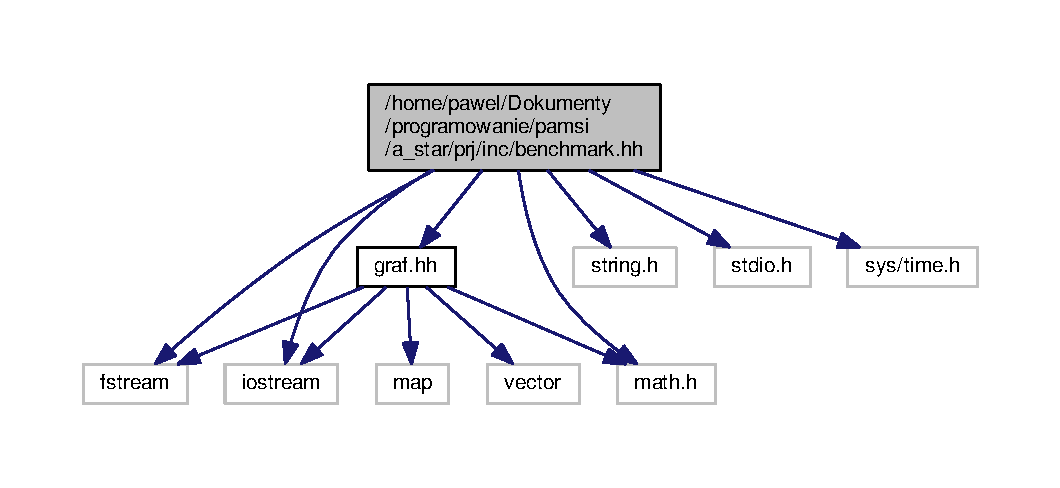
\includegraphics[width=350pt]{benchmark_8hh__incl}
\end{center}
\end{figure}
This graph shows which files directly or indirectly include this file\-:\nopagebreak
\begin{figure}[H]
\begin{center}
\leavevmode
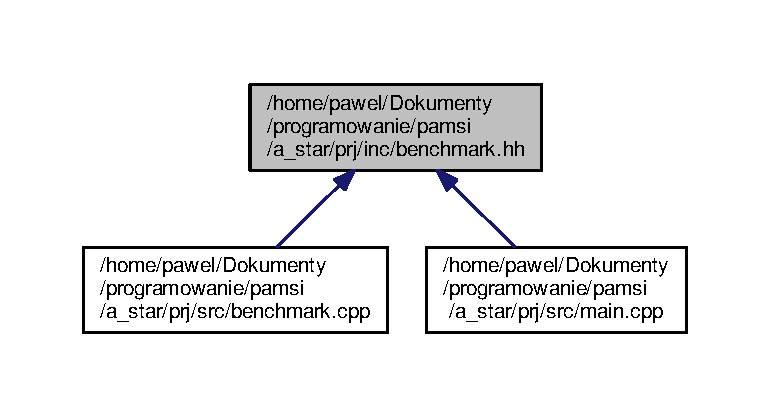
\includegraphics[width=350pt]{benchmark_8hh__dep__incl}
\end{center}
\end{figure}
\subsection*{Classes}
\begin{DoxyCompactItemize}
\item 
class \hyperlink{classbenchmark}{benchmark}
\begin{DoxyCompactList}\small\item\em Modeluje pojecie Benchmark. \end{DoxyCompactList}\end{DoxyCompactItemize}


\subsection{Detailed Description}
Definicje funkcji dla klasy benchmark. 

Definition in file \hyperlink{benchmark_8hh_source}{benchmark.\-hh}.


\hypertarget{graf_8hh}{\section{/home/pawel/\-Dokumenty/programowanie/pamsi/a\-\_\-star/prj/inc/graf.hh File Reference}
\label{graf_8hh}\index{/home/pawel/\-Dokumenty/programowanie/pamsi/a\-\_\-star/prj/inc/graf.\-hh@{/home/pawel/\-Dokumenty/programowanie/pamsi/a\-\_\-star/prj/inc/graf.\-hh}}
}


Definicje funkcji dla klasy graf.  


{\ttfamily \#include $<$iostream$>$}\\*
{\ttfamily \#include $<$vector$>$}\\*
{\ttfamily \#include $<$map$>$}\\*
{\ttfamily \#include $<$math.\-h$>$}\\*
{\ttfamily \#include $<$fstream$>$}\\*
Include dependency graph for graf.\-hh\-:\nopagebreak
\begin{figure}[H]
\begin{center}
\leavevmode
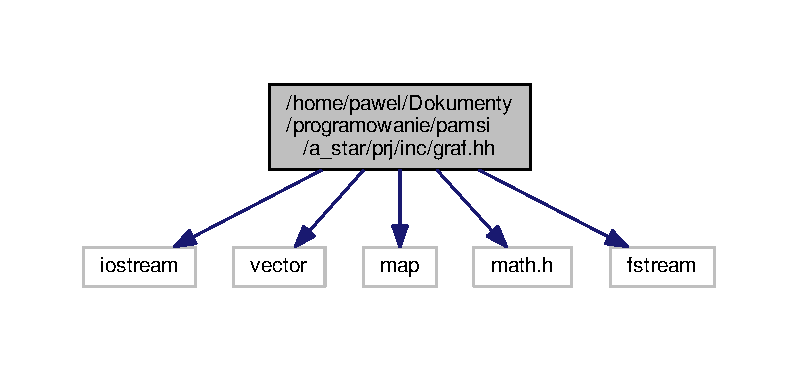
\includegraphics[width=350pt]{graf_8hh__incl}
\end{center}
\end{figure}
This graph shows which files directly or indirectly include this file\-:
\nopagebreak
\begin{figure}[H]
\begin{center}
\leavevmode
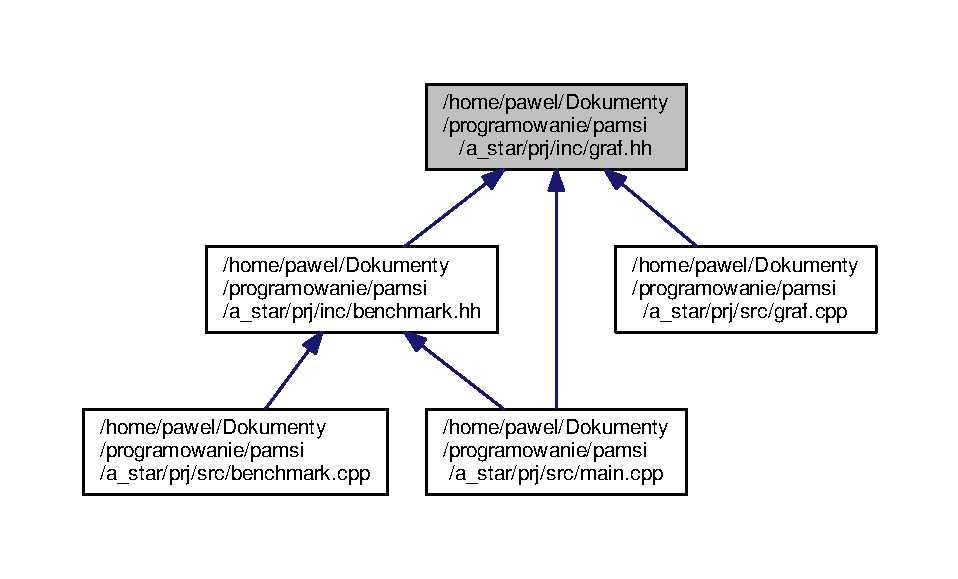
\includegraphics[width=350pt]{graf_8hh__dep__incl}
\end{center}
\end{figure}
\subsection*{Classes}
\begin{DoxyCompactItemize}
\item 
struct \hyperlink{struct_punkt}{Punkt}
\begin{DoxyCompactList}\small\item\em Struktura punktu Struktura ta ma zdefiniowane dwie zmienne x oraz y, ktore odpowiadaja za przechowywanie pozycji na siatce. Rowniez zdefiniowane sa operator przypisania oraz operator logiczny relacji. \end{DoxyCompactList}\item 
struct \hyperlink{struct_wierzcholek}{Wierzcholek}
\begin{DoxyCompactList}\small\item\em Struktura \hyperlink{struct_wierzcholek}{Wierzcholek}. Opisuje wlasnosci wierzcholka. \end{DoxyCompactList}\item 
class \hyperlink{classgraf}{graf}
\begin{DoxyCompactList}\small\item\em Modeluje pojecie graf. Klasa sluzy glownie do wykonania algorytmu a\-\_\-star, czyli znalezienia najlepszej drogi miedzy dwoma punktami. \end{DoxyCompactList}\end{DoxyCompactItemize}
\subsection*{Enumerations}
\begin{DoxyCompactItemize}
\item 
enum \hyperlink{graf_8hh_af54d448689b4613c3715929ca2a914a2}{Wierzcholek\-\_\-\-Typ} \{ \hyperlink{graf_8hh_af54d448689b4613c3715929ca2a914a2a846f623e19814cffb78d5ef92e77f7a3}{normalne}, 
\hyperlink{graf_8hh_af54d448689b4613c3715929ca2a914a2adb5535e159eca8e4dc5aafad57d8a4ba}{sciana}, 
\hyperlink{graf_8hh_af54d448689b4613c3715929ca2a914a2aeae5b57b7024c23312af9137b42aa6b1}{punkt}
 \}
\begin{DoxyCompactList}\small\item\em Rodzaje wierzcholkow Zdefiniowanie 3 roznych rodzajow wierzcholka \-: -\/$>$ normalne dla wierzcholkow wolnych, -\/$>$ sciana dla wierzcholkow bedacych przeszkodą, -\/$>$ punkt dla wierzcholkow, ktore sa punktami poczatkowymi i koncowymi. \end{DoxyCompactList}\end{DoxyCompactItemize}


\subsection{Detailed Description}
Definicje funkcji dla klasy graf. 

Definition in file \hyperlink{graf_8hh_source}{graf.\-hh}.



\subsection{Enumeration Type Documentation}
\hypertarget{graf_8hh_af54d448689b4613c3715929ca2a914a2}{\index{graf.\-hh@{graf.\-hh}!Wierzcholek\-\_\-\-Typ@{Wierzcholek\-\_\-\-Typ}}
\index{Wierzcholek\-\_\-\-Typ@{Wierzcholek\-\_\-\-Typ}!graf.hh@{graf.\-hh}}
\subsubsection[{Wierzcholek\-\_\-\-Typ}]{\setlength{\rightskip}{0pt plus 5cm}enum {\bf Wierzcholek\-\_\-\-Typ}}}\label{graf_8hh_af54d448689b4613c3715929ca2a914a2}


Rodzaje wierzcholkow Zdefiniowanie 3 roznych rodzajow wierzcholka \-: -\/$>$ normalne dla wierzcholkow wolnych, -\/$>$ sciana dla wierzcholkow bedacych przeszkodą, -\/$>$ punkt dla wierzcholkow, ktore sa punktami poczatkowymi i koncowymi. 

\begin{Desc}
\item[Enumerator]\par
\begin{description}
\index{normalne@{normalne}!graf.\-hh@{graf.\-hh}}\index{graf.\-hh@{graf.\-hh}!normalne@{normalne}}\item[{\em 
\hypertarget{graf_8hh_af54d448689b4613c3715929ca2a914a2a846f623e19814cffb78d5ef92e77f7a3}{normalne}\label{graf_8hh_af54d448689b4613c3715929ca2a914a2a846f623e19814cffb78d5ef92e77f7a3}
}]\index{sciana@{sciana}!graf.\-hh@{graf.\-hh}}\index{graf.\-hh@{graf.\-hh}!sciana@{sciana}}\item[{\em 
\hypertarget{graf_8hh_af54d448689b4613c3715929ca2a914a2adb5535e159eca8e4dc5aafad57d8a4ba}{sciana}\label{graf_8hh_af54d448689b4613c3715929ca2a914a2adb5535e159eca8e4dc5aafad57d8a4ba}
}]\index{punkt@{punkt}!graf.\-hh@{graf.\-hh}}\index{graf.\-hh@{graf.\-hh}!punkt@{punkt}}\item[{\em 
\hypertarget{graf_8hh_af54d448689b4613c3715929ca2a914a2aeae5b57b7024c23312af9137b42aa6b1}{punkt}\label{graf_8hh_af54d448689b4613c3715929ca2a914a2aeae5b57b7024c23312af9137b42aa6b1}
}]\end{description}
\end{Desc}


Definition at line 23 of file graf.\-hh.


\hypertarget{benchmark_8cpp}{\section{/home/pawel/\-Dokumenty/programowanie/pamsi/sortowaniev2/prj/src/benchmark.cpp File Reference}
\label{benchmark_8cpp}\index{/home/pawel/\-Dokumenty/programowanie/pamsi/sortowaniev2/prj/src/benchmark.\-cpp@{/home/pawel/\-Dokumenty/programowanie/pamsi/sortowaniev2/prj/src/benchmark.\-cpp}}
}


Plik zawiera funkcje z klasy benchmark.  


{\ttfamily \#include \char`\"{}../inc/benchmark.\-hh\char`\"{}}\\*
{\ttfamily \#include $<$iostream$>$}\\*
Include dependency graph for benchmark.\-cpp\-:\nopagebreak
\begin{figure}[H]
\begin{center}
\leavevmode
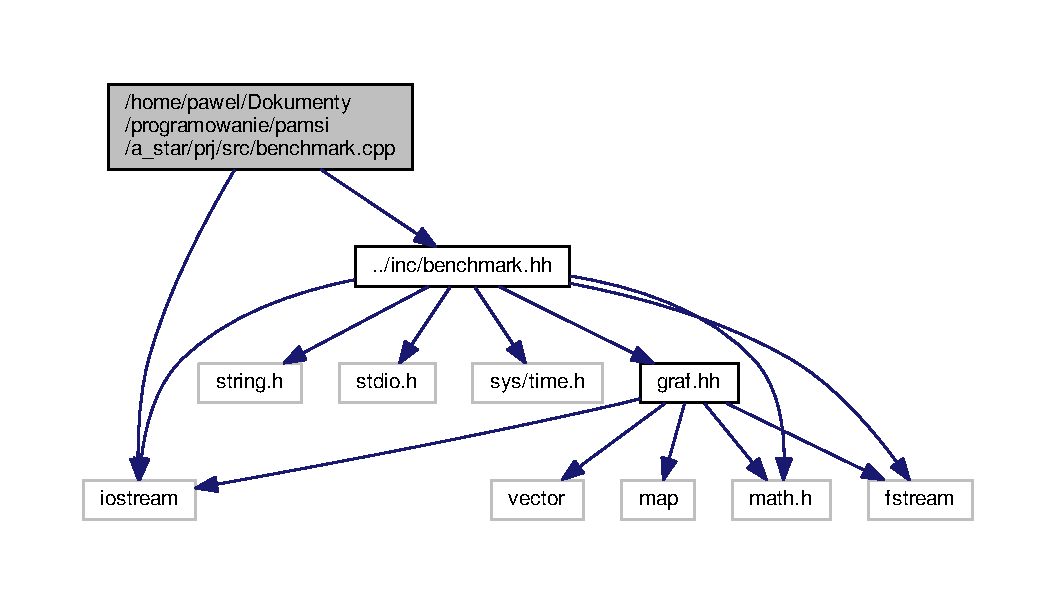
\includegraphics[width=350pt]{benchmark_8cpp__incl}
\end{center}
\end{figure}


\subsection{Detailed Description}
Plik zawiera funkcje z klasy benchmark. 

Definition in file \hyperlink{benchmark_8cpp_source}{benchmark.\-cpp}.


\hypertarget{graf_8cpp}{\section{/home/pawel/\-Dokumenty/programowanie/pamsi/a\-\_\-star/prj/src/graf.cpp File Reference}
\label{graf_8cpp}\index{/home/pawel/\-Dokumenty/programowanie/pamsi/a\-\_\-star/prj/src/graf.\-cpp@{/home/pawel/\-Dokumenty/programowanie/pamsi/a\-\_\-star/prj/src/graf.\-cpp}}
}


Plik zawiera funkcje z klasy graf.  


{\ttfamily \#include \char`\"{}../inc/graf.\-hh\char`\"{}}\\*
Include dependency graph for graf.\-cpp\-:\nopagebreak
\begin{figure}[H]
\begin{center}
\leavevmode
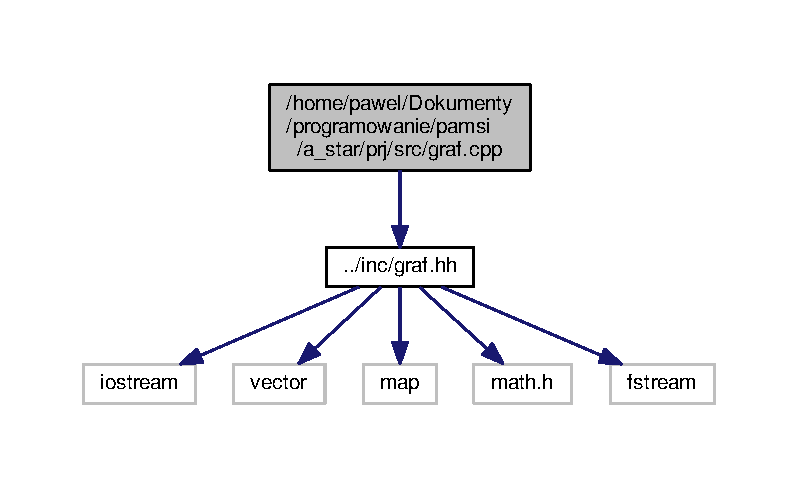
\includegraphics[width=350pt]{graf_8cpp__incl}
\end{center}
\end{figure}


\subsection{Detailed Description}
Plik zawiera funkcje z klasy graf. 

Definition in file \hyperlink{graf_8cpp_source}{graf.\-cpp}.


\hypertarget{main_8cpp}{\section{/home/pawel/\-Dokumenty/programowanie/pamsi/simplex/prj/src/main.cpp File Reference}
\label{main_8cpp}\index{/home/pawel/\-Dokumenty/programowanie/pamsi/simplex/prj/src/main.\-cpp@{/home/pawel/\-Dokumenty/programowanie/pamsi/simplex/prj/src/main.\-cpp}}
}


Plik zawiera funkcje \hyperlink{main_8cpp_ae66f6b31b5ad750f1fe042a706a4e3d4}{main()}  


{\ttfamily \#include $<$iostream$>$}\\*
{\ttfamily \#include \char`\"{}../inc/simplex.\-hh\char`\"{}}\\*
Include dependency graph for main.\-cpp\-:\nopagebreak
\begin{figure}[H]
\begin{center}
\leavevmode
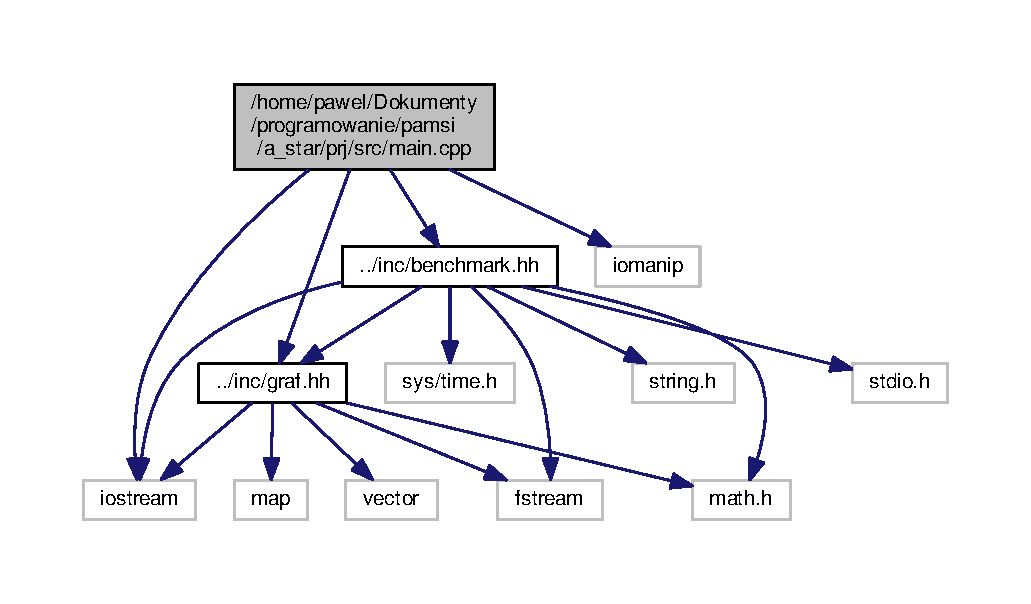
\includegraphics[width=224pt]{main_8cpp__incl}
\end{center}
\end{figure}
\subsection*{Functions}
\begin{DoxyCompactItemize}
\item 
int \hyperlink{main_8cpp_ae66f6b31b5ad750f1fe042a706a4e3d4}{main} ()
\end{DoxyCompactItemize}


\subsection{Detailed Description}
Plik zawiera funkcje \hyperlink{main_8cpp_ae66f6b31b5ad750f1fe042a706a4e3d4}{main()} 

Definition in file \hyperlink{main_8cpp_source}{main.\-cpp}.



\subsection{Function Documentation}
\hypertarget{main_8cpp_ae66f6b31b5ad750f1fe042a706a4e3d4}{\index{main.\-cpp@{main.\-cpp}!main@{main}}
\index{main@{main}!main.cpp@{main.\-cpp}}
\subsubsection[{main}]{\setlength{\rightskip}{0pt plus 5cm}int main (
\begin{DoxyParamCaption}
{}
\end{DoxyParamCaption}
)}}\label{main_8cpp_ae66f6b31b5ad750f1fe042a706a4e3d4}


Definition at line 13 of file main.\-cpp.



Here is the call graph for this function\-:\nopagebreak
\begin{figure}[H]
\begin{center}
\leavevmode
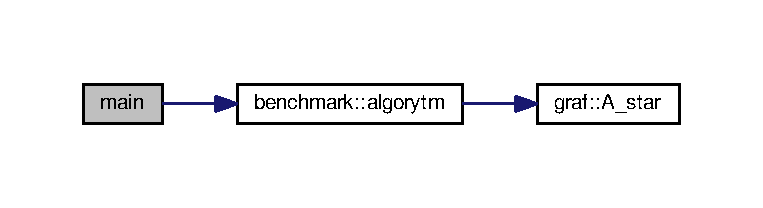
\includegraphics[width=282pt]{main_8cpp_ae66f6b31b5ad750f1fe042a706a4e3d4_cgraph}
\end{center}
\end{figure}



%--- End generated contents ---

% Index
\newpage
\phantomsection
\addcontentsline{toc}{chapter}{Index}
\printindex

\end{document}
